\begin{minipage}{0.75\linewidth}
\begin{figure}[h]
    \centering
    \begin{adjustbox}{max width=1.0\linewidth, keepaspectratio}
        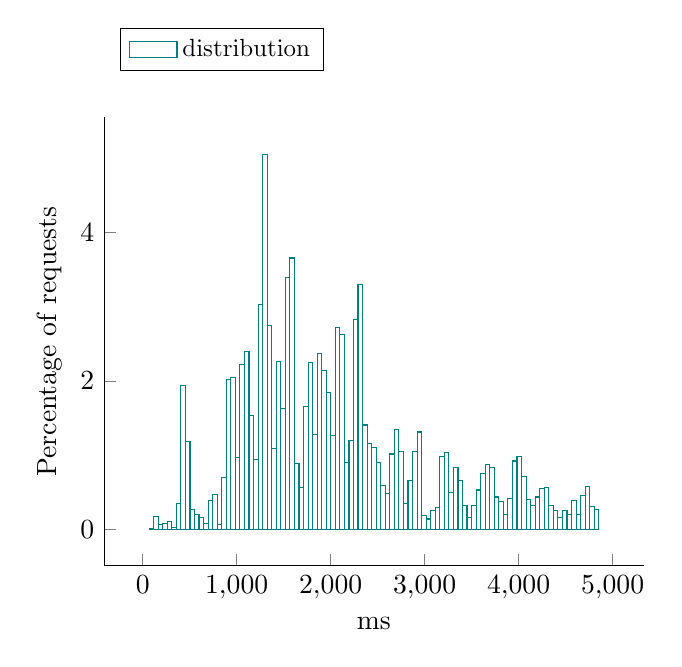
\begin{tikzpicture}
            \begin{axis}[ylabel = Percentage of requests, 
xlabel = ms, 
legend style = {nodes={scale=0.9, transform shape}, at={(0.03,1.2)}, anchor=north west, draw=black, fill=white, align=left, legend columns=3},
area style, mark size = 0pt,
 cycle list name = exotic,
  axis lines* = left]
		\addplot +[ybar interval] coordinates {
			 (68, 0.015625)
			 (116.33, 0.171875)
			 (164.66, 0.0625)
			 (212.99, 0.078125)
			 (261.32, 0.109375)
			 (309.65, 0.03125)
			 (357.98, 0.34375)
			 (406.31, 1.9375)
			 (454.64, 1.1875)
			 (502.97, 0.265625)
			 (551.3, 0.203125)
			 (599.63, 0.15625)
			 (647.96, 0.078125)
			 (696.29, 0.390625)
			 (744.62, 0.46875)
			 (792.95, 0.0625)
			 (841.28, 0.703125)
			 (889.61, 2.01562)
			 (937.94, 2.04688)
			 (986.27, 0.96875)
			 (1034.6, 2.21875)
			 (1082.93, 2.39062)
			 (1131.26, 1.53125)
			 (1179.59, 0.9375)
			 (1227.92, 3.03125)
			 (1276.25, 5.04688)
			 (1324.58, 2.75)
			 (1372.91, 1.09375)
			 (1421.24, 2.26562)
			 (1469.57, 1.625)
			 (1517.9, 3.39062)
			 (1566.23, 3.65625)
			 (1614.56, 0.890625)
			 (1662.89, 0.5625)
			 (1711.22, 1.65625)
			 (1759.55, 2.25)
			 (1807.88, 1.28125)
			 (1856.21, 2.375)
			 (1904.54, 2.14062)
			 (1952.87, 1.84375)
			 (2001.2, 1.26562)
			 (2049.53, 2.71875)
			 (2097.86, 2.625)
			 (2146.19, 0.90625)
			 (2194.52, 1.20312)
			 (2242.85, 2.82812)
			 (2291.18, 3.29688)
			 (2339.51, 1.40625)
			 (2387.84, 1.15625)
			 (2436.17, 1.10938)
			 (2484.5, 0.90625)
			 (2532.83, 0.59375)
			 (2581.16, 0.484375)
			 (2629.49, 1.01562)
			 (2677.82, 1.34375)
			 (2726.15, 1.04688)
			 (2774.48, 0.34375)
			 (2822.81, 0.65625)
			 (2871.14, 1.04688)
			 (2919.47, 1.3125)
			 (2967.8, 0.1875)
			 (3016.13, 0.140625)
			 (3064.46, 0.25)
			 (3112.79, 0.296875)
			 (3161.12, 0.984375)
			 (3209.45, 1.03125)
			 (3257.78, 0.5)
			 (3306.11, 0.828125)
			 (3354.44, 0.65625)
			 (3402.77, 0.328125)
			 (3451.1, 0.15625)
			 (3499.43, 0.328125)
			 (3547.76, 0.53125)
			 (3596.09, 0.75)
			 (3644.42, 0.875)
			 (3692.75, 0.828125)
			 (3741.08, 0.4375)
			 (3789.41, 0.375)
			 (3837.74, 0.203125)
			 (3886.07, 0.421875)
			 (3934.4, 0.921875)
			 (3982.73, 0.984375)
			 (4031.06, 0.71875)
			 (4079.39, 0.40625)
			 (4127.72, 0.328125)
			 (4176.05, 0.4375)
			 (4224.38, 0.546875)
			 (4272.71, 0.5625)
			 (4321.04, 0.328125)
			 (4369.37, 0.25)
			 (4417.7, 0.15625)
			 (4466.03, 0.25)
			 (4514.36, 0.203125)
			 (4562.69, 0.390625)
			 (4611.02, 0.203125)
			 (4659.35, 0.453125)
			 (4707.68, 0.578125)
			 (4756.01, 0.3125)
			 (4804.34, 0.265625)
			 (4852.67, 0.078125)
		};
\addlegendentry{distribution};
           \end{axis}
      \end{tikzpicture}
  \end{adjustbox}
  \caption{Response time distribution - req = ReadTimeline-1}
\end{figure}
\end{minipage}\hfill\begin{minipage}{0.18\linewidth}
\begin{table}[h]
\begin{tabular}{|cc|}
\hline
\textbf{} & \textbf{ms}\\ \hline
 \Xhline{0.005\arrayrulewidth}
min & 68\\
 \Xhline{0.005\arrayrulewidth}
max & 4901\\
 \Xhline{0.005\arrayrulewidth}
mean & 2087\\
 \Xhline{0.005\arrayrulewidth}
std & 1033\\
\hline
\hline
 \Xhline{0.005\arrayrulewidth}
25th & 1311\\
 \Xhline{0.005\arrayrulewidth}
50th & 1900\\
 \Xhline{0.005\arrayrulewidth}
75th & 2654\\
 \Xhline{0.005\arrayrulewidth}
80th & 2915\\
 \Xhline{0.005\arrayrulewidth}
85th & 3316\\
 \Xhline{0.005\arrayrulewidth}
90th & 3732\\
 \Xhline{0.005\arrayrulewidth}
95th & 4185\\
 \Xhline{0.005\arrayrulewidth}
99th & 4722\\
\hline
\end{tabular}
\caption{Response time}
\end{table}
\end{minipage}\hfill